\documentclass[12pt,a4paper]{article}

\usepackage[T1]{fontenc}
\usepackage{amsmath}
\usepackage{amssymb}
\usepackage{amsthm}
\usepackage[margin=2.5cm]{geometry}
\usepackage{hyperref}
\usepackage[dvipsnames]{xcolor}
\usepackage{tikz}
\usepackage{pgfplots}
\pgfplotsset{compat=1.18}
\usepackage{tcolorbox}
\usepackage{booktabs}
\usepackage{array}
\usepackage{enumitem}
\usepackage{fancyhdr}
\usepackage{titlesec}
\usepackage{microtype}
\usepackage{setspace}

\setlength{\headheight}{14pt}

\usetikzlibrary{arrows.meta,calc,positioning,shapes.geometric,decorations.pathreplacing,backgrounds,fit,matrix}

\pagestyle{fancy}
\fancyhf{}
\rhead{\small Linear Transformations}
\lhead{\small Lecture Notes}
\cfoot{\thepage}

\newcommand{\R}{\mathbb{R}}
\newcommand{\N}{\mathbb{N}}
\newcommand{\C}{\mathbb{C}}
\newcommand{\Z}{\mathbb{Z}}
\newcommand{\Q}{\mathbb{Q}}
\newcommand{\vv}[1]{\mathbf{#1}}
\newcommand{\vzero}{\mathbf{0}}
\newcommand{\Span}{\text{Span}}
\newcommand{\rank}{\text{rank}}
\newcommand{\nullity}{\text{nullity}}
\newcommand{\im}{\text{im}}

\tcbset{
	defstyle/.style={
		colback=Blue!5,
		colframe=Blue!75!black,
		arc=0mm,
		boxrule=1.5pt,
		left=5pt,
		right=5pt,
		top=5pt,
		bottom=5pt,
		fonttitle=\bfseries,
		title={#1}
	},
	thmstyle/.style={
		colback=Cyan!5,
		colframe=Cyan!75!black,
		arc=0mm,
		boxrule=1.5pt,
		left=5pt,
		right=5pt,
		top=5pt,
		bottom=5pt,
		fonttitle=\bfseries,
		title={#1}
	},
	exstyle/.style={
		colback=Yellow!10,
		colframe=Orange!75!black,
		arc=0mm,
		boxrule=1.5pt,
		left=5pt,
		right=5pt,
		top=5pt,
		bottom=5pt,
		fonttitle=\bfseries,
		title={#1}
	},
	remstyle/.style={
		colback=Red!5,
		colframe=Red!75!black,
		arc=0mm,
		boxrule=1.5pt,
		left=5pt,
		right=5pt,
		top=5pt,
		bottom=5pt,
		fonttitle=\bfseries,
		title={#1}
	},
	propstyle/.style={
		colback=Green!5,
		colframe=Green!75!black,
		arc=0mm,
		boxrule=1.5pt,
		left=5pt,
		right=5pt,
		top=5pt,
		bottom=5pt,
		fonttitle=\bfseries,
		title={#1}
	}
}

\newtcolorbox{definition}[1]{defstyle={Definition: #1}}
\newtcolorbox{theorem}[1]{thmstyle={Theorem: #1}}
\newtcolorbox{example}[1]{exstyle={Example: #1}}
\newtcolorbox{remark}[1]{remstyle={Remark: #1}}
\newtcolorbox{proposition}[1]{propstyle={Proposition: #1}}
\newtcolorbox{proofbox}{
	colback=White,
	colframe=Black!50,
	arc=0mm,
	boxrule=0.8pt,
	left=5pt,
	right=5pt,
	top=5pt,
	bottom=5pt,
	fonttitle=\bfseries,
	title={Proof}
}

\titleformat{\section}{\Large\bfseries\color{Blue!75!black}}{}{0em}{}[\vspace{0.2cm}\hrule\vspace{0.2cm}]
\titleformat{\subsection}{\large\bfseries\color{Cyan!75!black}}{}{0em}{}

\onehalfspacing

\title{\textbf{Linear Transformations}}
\author{Lecture Notes}
\date{\today}

\begin{document}
	
	\maketitle
	
	\tableofcontents
	
	\newpage
	
	\section{Introduction to Linear Transformations}
	
	Linear mappings from one vector space to another play an important role in mathematics. This chapter provides an introduction to the theory of such mappings. 
	
	Linear transformations are fundamental tools in linear algebra that allow us to study the structure and relationships between vector spaces. By understanding how linear transformations work, we can solve many practical problems in mathematics, physics, engineering, and computer science.
	
	In this chapter, we will explore several key topics:
	
	\begin{itemize}
		\item The definition of linear transformations and various examples
		\item Matrix representation of linear transformations
		\item Relationships between different matrix representations
		\item The kernel and image of linear transformations
		\item Applications to geometric transformations and beyond
	\end{itemize}
	
	The theory developed here shows that every linear transformation from an $n$-dimensional vector space $V$ into an $m$-dimensional vector space $W$ can be represented by an $m \times n$ matrix. This allows us to work with matrices instead of abstract transformations, making computations more tractable.
	
	\section{Linear Operators on $\R^2$}
	
	Linear transformations on $\R^2$ provide intuitive geometric examples. A linear transformation $L: \R^2 \to \R^2$ is called a linear operator on $\R^2$.
	
	\begin{definition}{Linear Operator on $\R^2$}
		A function $L: \R^2 \to \R^2$ is a linear operator if for all vectors $\vv{u}, \vv{v} \in \R^2$ and all scalars $c \in \R$:
		\begin{enumerate}[label=(\roman*)]
			\item $L(\vv{u} + \vv{v}) = L(\vv{u}) + L(\vv{v})$ \quad (additivity)
			\item $L(c\vv{u}) = cL(\vv{u})$ \quad (homogeneity)
		\end{enumerate}
	\end{definition}
	
	\begin{example}{Rotation in R2}
		The counterclockwise rotation by angle $\theta$ is given by:
		\[
		L\begin{pmatrix} x \\ y \end{pmatrix} = \begin{pmatrix} \cos\theta & -\sin\theta \\ \sin\theta & \cos\theta \end{pmatrix} \begin{pmatrix} x \\ y \end{pmatrix} = \begin{pmatrix} x\cos\theta - y\sin\theta \\ x\sin\theta + y\cos\theta \end{pmatrix}
		\]
		This is a linear operator on $\R^2$.
		
		\textbf{Verification:} Let $\vv{u} = \begin{pmatrix} u_1 \\ u_2 \end{pmatrix}$ and $\vv{v} = \begin{pmatrix} v_1 \\ v_2 \end{pmatrix}$.
		
		Additivity: 
		\begin{align*}
			L(\vv{u} + \vv{v}) &= L\begin{pmatrix} u_1 + v_1 \\ u_2 + v_2 \end{pmatrix} \\
			&= \begin{pmatrix} \cos\theta & -\sin\theta \\ \sin\theta & \cos\theta \end{pmatrix} \begin{pmatrix} u_1 + v_1 \\ u_2 + v_2 \end{pmatrix} \\
			&= \begin{pmatrix} (u_1 + v_1)\cos\theta - (u_2 + v_2)\sin\theta \\ (u_1 + v_1)\sin\theta + (u_2 + v_2)\cos\theta \end{pmatrix} \\
			&= \begin{pmatrix} u_1\cos\theta - u_2\sin\theta \\ u_1\sin\theta + u_2\cos\theta \end{pmatrix} + \begin{pmatrix} v_1\cos\theta - v_2\sin\theta \\ v_1\sin\theta + v_2\cos\theta \end{pmatrix} \\
			&= L(\vv{u}) + L(\vv{v})
		\end{align*}
		
		Homogeneity: For scalar $c$,
		\begin{align*}
			L(c\vv{u}) &= L\begin{pmatrix} cu_1 \\ cu_2 \end{pmatrix} \\
			&= \begin{pmatrix} cu_1\cos\theta - cu_2\sin\theta \\ cu_1\sin\theta + cu_2\cos\theta \end{pmatrix} \\
			&= c\begin{pmatrix} u_1\cos\theta - u_2\sin\theta \\ u_1\sin\theta + u_2\cos\theta \end{pmatrix} \\
			&= cL(\vv{u})
		\end{align*}
		
		Thus, rotation is indeed a linear operator.
	\end{example}
	
	\begin{example}{Reflection across the x-axis}
		The reflection across the $x$-axis is given by:
		\[
		L\begin{pmatrix} x \\ y \end{pmatrix} = \begin{pmatrix} 1 & 0 \\ 0 & -1 \end{pmatrix} \begin{pmatrix} x \\ y \end{pmatrix} = \begin{pmatrix} x \\ -y \end{pmatrix}
		\]
		This transformation is linear. For instance, if we reflect the point $(3, 4)$, we get $L\begin{pmatrix} 3 \\ 4 \end{pmatrix} = \begin{pmatrix} 3 \\ -4 \end{pmatrix}$.
	\end{example}
	
	\begin{example}{Scaling (Dilation)}
		Scaling by a factor of $k > 0$ is given by:
		\[
		L\begin{pmatrix} x \\ y \end{pmatrix} = \begin{pmatrix} k & 0 \\ 0 & k \end{pmatrix} \begin{pmatrix} x \\ y \end{pmatrix} = \begin{pmatrix} kx \\ ky \end{pmatrix}
		\]
		For example, scaling by $k = 2$ doubles all distances from the origin. This is also a linear operator.
	\end{example}
	
	\begin{example}{Shear Transformation with Geometric Representation}
		A shear transformation in the $x$-direction is given by:
		\[
		L\begin{pmatrix} x \\ y \end{pmatrix} = \begin{pmatrix} 1 & a \\ 0 & 1 \end{pmatrix} \begin{pmatrix} x \\ y \end{pmatrix} = \begin{pmatrix} x + ay \\ y \end{pmatrix}
		\]
		where $a$ is the shear parameter. This transformation moves points to the right by an amount proportional to their $y$-coordinate, while leaving the $y$-coordinate unchanged.
		
		For example, with $a = 0.5$:
		\begin{align*}
			L\begin{pmatrix} 1 \\ 0 \end{pmatrix} &= \begin{pmatrix} 1 \\ 0 \end{pmatrix} \\
			L\begin{pmatrix} 0 \\ 1 \end{pmatrix} &= \begin{pmatrix} 0.5 \\ 1 \end{pmatrix} \\
			L\begin{pmatrix} 1 \\ 1 \end{pmatrix} &= \begin{pmatrix} 1.5 \\ 1 \end{pmatrix}
		\end{align*}
		
		\textbf{Geometric Representation:}
		
		\begin{center}
			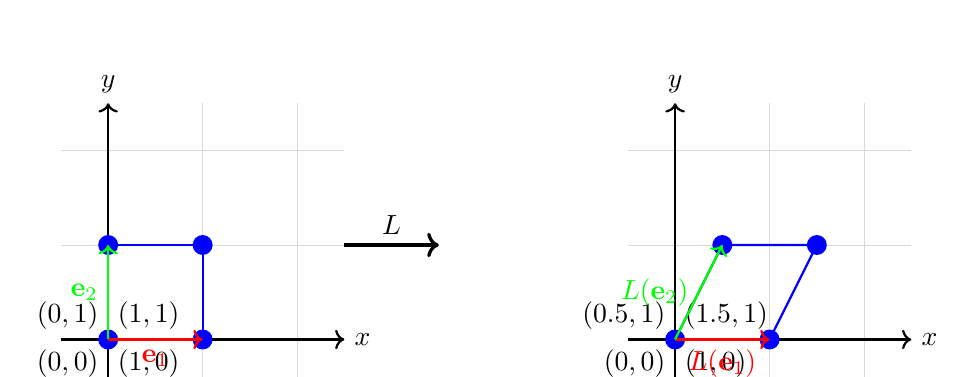
\begin{tikzpicture}[scale=1.2]
				
				\begin{scope}[shift={(-4,0)}]
					
					\draw[help lines, gray!30] (-0.5,-0.5) grid (2.5,2.5);
					
					
					\draw[thick, ->] (-0.5,0) -- (2.5,0) node[right] {$x$};
					\draw[thick, ->] (0,-0.5) -- (0,2.5) node[above] {$y$};
					
					
					\draw[blue, thick] (0,0) -- (1,0) -- (1,1) -- (0,1) -- cycle;
					
				
					\fill[blue] (0,0) circle (3pt);
					\node[below left] {$(0,0)$};
					\fill[blue] (1,0) circle (3pt);
					\node[below right] {$(1,0)$};
					\fill[blue] (1,1) circle (3pt);
					\node[above right] {$(1,1)$};
					\fill[blue] (0,1) circle (3pt);
					\node[above left] {$(0,1)$};
					
				
					\draw[red, thick, ->] (0,0) -- (1,0) node[midway, below] {$\vv{e}_1$};
					\draw[green, thick, ->] (0,0) -- (0,1) node[midway, left] {$\vv{e}_2$};
					
					
				\end{scope}
				
				
				\begin{scope}[shift={(2,0)}]
				
					\draw[help lines, gray!30] (-0.5,-0.5) grid (2.5,2.5);
					
					
					\draw[thick, ->] (-0.5,0) -- (2.5,0) node[right] {$x$};
					\draw[thick, ->] (0,-0.5) -- (0,2.5) node[above] {$y$};
					
				
					\draw[blue, thick] (0,0) -- (1,0) -- (1.5,1) -- (0.5,1) -- cycle;
					
					
					\fill[blue] (0,0) circle (3pt);
					\node[below left] {$(0,0)$};
					\fill[blue] (1,0) circle (3pt);
					\node[below right] {$(1,0)$};
					\fill[blue] (1.5,1) circle (3pt);
					\node[above right] {$(1.5,1)$};
					\fill[blue] (0.5,1) circle (3pt);
					\node[above left] {$(0.5,1)$};
					
					
					\draw[red, thick, ->] (0,0) -- (1,0) node[midway, below] {$L(\vv{e}_1)$};
					\draw[green, thick, ->] (0,0) -- (0.5,1) node[midway, left] {$L(\vv{e}_2)$};
					
					
				\end{scope}
				
			
				\draw[->, very thick, black] (-1.5, 1) -- (-0.5, 1) node[midway, above] {$L$};
			\end{tikzpicture}
		\end{center}
		
		\textbf{Verification of Linearity:} We verify that the shear transformation satisfies the linearity properties. For additivity:
		\begin{align*}
			L(\vv{u} + \vv{v}) &= L\begin{pmatrix} u_1 + v_1 \\ u_2 + v_2 \end{pmatrix} \\
			&= \begin{pmatrix} (u_1 + v_1) + a(u_2 + v_2) \\ u_2 + v_2 \end{pmatrix} \\
			&= \begin{pmatrix} u_1 + au_2 \\ u_2 \end{pmatrix} + \begin{pmatrix} v_1 + av_2 \\ v_2 \end{pmatrix} \\
			&= L(\vv{u}) + L(\vv{v})
		\end{align*}
		
		For homogeneity:
		\begin{align*}
			L(c\vv{u}) &= L\begin{pmatrix} cu_1 \\ cu_2 \end{pmatrix} \\
			&= \begin{pmatrix} cu_1 + a(cu_2) \\ cu_2 \end{pmatrix} \\
			&= c\begin{pmatrix} u_1 + au_2 \\ u_2 \end{pmatrix} \\
			&= cL(\vv{u})
		\end{align*}
		
		Thus, the shear transformation is linear.
		
		\textbf{Geometric Interpretation:} The shear transformation preserves horizontal and vertical lines, preserves areas (the determinant of the matrix is $1$), and ``tilts'' the coordinate system. The unit square becomes a parallelogram.
	\end{example}
	
	\begin{remark}{Geometric Intuition}
		Linear transformations in $\R^2$ preserve the origin (since $L(\vzero) = \vzero$), map lines to lines or the origin, and preserve parallelograms. These properties can be verified algebraically using the definition of linearity. The visualizations above show how different linear transformations distort the plane in characteristic ways.
	\end{remark}
	
	\section{Linear Transformations from Rn to Rm}
	
	We now generalize the concept of linear transformations to mappings between general Euclidean spaces.
	
	\begin{definition}{Linear Transformation}
		A function $L: \R^n \to \R^m$ is a linear transformation if for all vectors $\vv{u}, \vv{v} \in \R^n$ and all scalars $c \in \R$:
		\begin{enumerate}[label=(\roman*)]
			\item $L(\vv{u} + \vv{v}) = L(\vv{u}) + L(\vv{v})$ \quad (additivity)
			\item $L(c\vv{u}) = cL(\vv{u})$ \quad (homogeneity)
		\end{enumerate}
	\end{definition}
	
	\begin{remark}{Equivalent Characterization}
		A function $L: \R^n \to \R^m$ is linear if and only if:
		\[
		L(c_1\vv{u}_1 + c_2\vv{u}_2 + \cdots + c_k\vv{u}_k) = c_1L(\vv{u}_1) + c_2L(\vv{u}_2) + \cdots + c_kL(\vv{u}_k)
		\]
		for all vectors $\vv{u}_1, \vv{u}_2, \ldots, \vv{u}_k \in \R^n$ and all scalars $c_1, c_2, \ldots, c_k \in \R$. 
		
		In particular, $L(\vzero) = \vzero$ (the zero vector maps to the zero vector).
	\end{remark}
	
	\begin{example}{Matrix-Induced Linear Transformation}
		Let $A$ be an $m \times n$ matrix. The function $L(\vv{x}) = A\vv{x}$ is a linear transformation from $\R^n$ to $\R^m$. This is because:
		\[
		L(c_1\vv{x}_1 + c_2\vv{x}_2) = A(c_1\vv{x}_1 + c_2\vv{x}_2) = c_1A\vv{x}_1 + c_2A\vv{x}_2 = c_1L(\vv{x}_1) + c_2L(\vv{x}_2)
		\]
	\end{example}
	
	\begin{example}{Projection onto the xy-plane}
		Consider $L: \R^3 \to \R^3$ defined by $L(x, y, z) = (x, y, 0)$. This projects any point onto the $xy$-plane.
		
		Represented as a matrix:
		\[
		L\begin{pmatrix} x \\ y \\ z \end{pmatrix} = \begin{pmatrix} 1 & 0 & 0 \\ 0 & 1 & 0 \\ 0 & 0 & 0 \end{pmatrix} \begin{pmatrix} x \\ y \\ z \end{pmatrix} = \begin{pmatrix} x \\ y \\ 0 \end{pmatrix}
		\]
		
		For example:
		\[
		L\begin{pmatrix} 2 \\ 3 \\ 5 \end{pmatrix} = \begin{pmatrix} 2 \\ 3 \\ 0 \end{pmatrix}
		\]
		
		This is linear: for any vectors and scalars, the sum and scalar multiplication properties are satisfied.
	\end{example}
	
	\begin{example}{Differentiation Operator}
		Consider the vector space $P_2$ of polynomials of degree at most 2. Define $L: P_2 \to P_1$ by $L(p(x)) = p'(x)$ (differentiation).
		
		For example:
		\begin{align*}
			L(3x^2 + 2x + 1) &= 6x + 2 \\
			L(5x^2 - 3) &= 10x
		\end{align*}
		
		This is linear because:
		\begin{align*}
			L(p + q) &= (p + q)' = p' + q' = L(p) + L(q) \\
			L(cp) &= (cp)' = cp' = cL(p)
		\end{align*}
	\end{example}
	
	\newpage
	
	\section{Linear Transformations from V to W}
	
	The concepts of linear transformations extend naturally to general vector spaces.
	
	\begin{definition}{Linear Transformation (General Spaces)}
		Let $V$ and $W$ be vector spaces over the same field. A function $L: V \to W$ is a linear transformation if for all vectors $\vv{v}_1, \vv{v}_2 \in V$ and all scalars $c$:
		\begin{enumerate}[label=(\roman*)]
			\item $L(\vv{v}_1 + \vv{v}_2) = L(\vv{v}_1) + L(\vv{v}_2)$
			\item $L(c\vv{v}_1) = cL(\vv{v}_1)$
		\end{enumerate}
	\end{definition}
	
	\begin{proposition}{Properties of Linear Transformations}
		Let $L: V \to W$ be a linear transformation. Then:
		\begin{enumerate}[label=(\roman*)]
			\item $L(\vzero_V) = \vzero_W$, where $\vzero_V$ and $\vzero_W$ are the zero vectors in $V$ and $W$, respectively.
			\item $L(-\vv{v}) = -L(\vv{v})$ for all $\vv{v} \in V$.
			\item $L(c_1\vv{v}_1 + c_2\vv{v}_2 + \cdots + c_k\vv{v}_k) = c_1L(\vv{v}_1) + c_2L(\vv{v}_2) + \cdots + c_kL(\vv{v}_k)$ for all vectors and scalars.
		\end{enumerate}
	\end{proposition}
	
	\subsection{The Image and Kernel}
	
	Two fundamental subspaces associated with a linear transformation are its image (range) and kernel (null space).
	
	\begin{definition}{Image and Kernel}
		Let $L: V \to W$ be a linear transformation.
		
		The \textbf{image} (or \textbf{range}) of $L$ is:
		\[
		\im(L) = L(V) = \{L(\vv{v}) : \vv{v} \in V\}
		\]
		
		The \textbf{kernel} (or \textbf{null space}) of $L$ is:
		\[
		\ker(L) = \{\vv{v} \in V : L(\vv{v}) = \vzero_W\}
		\]
	\end{definition}
	
	\begin{theorem}{Kernel and Image are Subspaces}
		Let $L: V \to W$ be a linear transformation and let $S$ be a subspace of $V$. Then:
		\begin{enumerate}[label=(\roman*)]
			\item $\ker(L)$ is a subspace of $V$.
			\item $L(S)$ is a subspace of $W$.
		\end{enumerate}
	\end{theorem}
	
	\begin{proofbox}
		
		\textbf{Proof of (i):} We show that $\ker(L)$ is nonempty and closed under scalar multiplication and vector addition.
		
		First, observe that $\ker(L)$ is nonempty since the zero vector $\vzero_V \in \ker(L)$, as $L(\vzero_V) = \vzero_W$ (a property of linear transformations).
		
		\textbf{Closure under scalar multiplication:} Let $\vv{v} \in \ker(L)$ and let $\alpha$ be a scalar. Then:
		\[
		L(\alpha\vv{v}) = \alpha L(\vv{v}) = \alpha \vzero_W = \vzero_W
		\]
		Therefore, $\alpha\vv{v} \in \ker(L)$.
		
		\textbf{Closure under addition:} Let $\vv{v}_1, \vv{v}_2 \in \ker(L)$. Then:
		\[
		L(\vv{v}_1 + \vv{v}_2) = L(\vv{v}_1) + L(\vv{v}_2) = \vzero_W + \vzero_W = \vzero_W
		\]
		Therefore, $\vv{v}_1 + \vv{v}_2 \in \ker(L)$, and hence $\ker(L)$ is a subspace of $V$.
		
		\textbf{Proof of (ii):} We show that $L(S)$ is nonempty and closed under scalar multiplication and vector addition.
		
		First, $L(S)$ is nonempty since $\vzero_W = L(\vzero_V) \in L(S)$ (as $\vzero_V \in S$).
		
		\textbf{Closure under scalar multiplication:} If $\vv{w} \in L(S)$, then $\vv{w} = L(\vv{v})$ for some $\vv{v} \in S$. For any scalar $\alpha$:
		\[
		\alpha\vv{w} = \alpha L(\vv{v}) = L(\alpha\vv{v})
		\]
		Since $S$ is a subspace and $\vv{v} \in S$, we have $\alpha\vv{v} \in S$. Therefore, $\alpha\vv{w} \in L(S)$, and $L(S)$ is closed under scalar multiplication.
		
		\textbf{Closure under addition:} If $\vv{w}_1, \vv{w}_2 \in L(S)$, then there exist $\vv{v}_1, \vv{v}_2 \in S$ such that $L(\vv{v}_1) = \vv{w}_1$ and $L(\vv{v}_2) = \vv{w}_2$. Thus:
		\[
		\vv{w}_1 + \vv{w}_2 = L(\vv{v}_1) + L(\vv{v}_2) = L(\vv{v}_1 + \vv{v}_2)
		\]
		Since $S$ is a subspace and $\vv{v}_1, \vv{v}_2 \in S$, we have $\vv{v}_1 + \vv{v}_2 \in S$. Therefore, $\vv{w}_1 + \vv{w}_2 \in L(S)$, and hence $L(S)$ is closed under addition. It follows that $L(S)$ is a subspace of $W$.
		
	\end{proofbox}
	
	\begin{remark}{Importance of Kernel and Image}
		The kernel and image of a linear transformation are central to understanding its behavior. The kernel tells us which vectors are ``collapsed'' to the zero vector, while the image tells us which vectors in $W$ are actually attained by the transformation. These concepts are essential for analyzing injectivity and surjectivity of linear transformations.
	\end{remark}
	
	\begin{example}{Kernel and Image of a Matrix Transformation}
		Let $A = \begin{pmatrix} 1 & 2 & 0 \\ 0 & 0 & 1 \end{pmatrix}$ and consider $L: \R^3 \to \R^2$ defined by $L(\vv{x}) = A\vv{x}$.
		
		\textbf{Finding the kernel:} The kernel of $L$ consists of all $\vv{x} = \begin{pmatrix} x_1 \\ x_2 \\ x_3 \end{pmatrix}$ such that:
		\[
		\begin{pmatrix} 1 & 2 & 0 \\ 0 & 0 & 1 \end{pmatrix} \begin{pmatrix} x_1 \\ x_2 \\ x_3 \end{pmatrix} = \begin{pmatrix} 0 \\ 0 \end{pmatrix}
		\]
		
		This gives us the system:
		\begin{align*}
			x_1 + 2x_2 &= 0 \\
			x_3 &= 0
		\end{align*}
		
		From the first equation, $x_1 = -2x_2$. Let $x_2 = t$ (a free variable). Then:
		\[
		\vv{x} = \begin{pmatrix} -2t \\ t \\ 0 \end{pmatrix} = t\begin{pmatrix} -2 \\ 1 \\ 0 \end{pmatrix}
		\]
		
		Therefore:
		\[
		\ker(L) = \Span\left\{\begin{pmatrix} -2 \\ 1 \\ 0 \end{pmatrix}\right\}
		\]
		
		\textbf{Finding the image:} The image of $L$ consists of all vectors that can be written as $A\vv{x}$ for some $\vv{x} \in \R^3$. The image is spanned by the columns of $A$:
		\[
		\im(L) = \Span\left\{\begin{pmatrix} 1 \\ 0 \end{pmatrix}, \begin{pmatrix} 2 \\ 0 \end{pmatrix}, \begin{pmatrix} 0 \\ 1 \end{pmatrix}\right\}
		\]
		
		Since the second column is $2$ times the first column, we can eliminate it:
		\[
		\im(L) = \Span\left\{\begin{pmatrix} 1 \\ 0 \end{pmatrix}, \begin{pmatrix} 0 \\ 1 \end{pmatrix}\right\} = \R^2
		\]
		
		So the transformation is surjective (maps onto $\R^2$).
	\end{example}
	
	\begin{example}{Kernel and Image of the Zero Transformation}
		Let $L: \R^3 \to \R^2$ be the zero transformation, defined by $L(\vv{x}) = \vzero$ for all $\vv{x} \in \R^3$.
		
		\textbf{Kernel:} $\ker(L) = \R^3$ (all vectors map to zero).
		
		\textbf{Image:} $\im(L) = \{\vzero\}$ (only the zero vector is in the image).
		
		This demonstrates the extreme cases where the kernel is the entire domain and the image is trivial.
	\end{example}
	
	\begin{example}{Kernel and Image of a Projection}
		Let $L: \R^3 \to \R^3$ be the projection onto the $xy$-plane, defined by $L(x, y, z) = (x, y, 0)$.
		
		The matrix representation is:
		\[
		A = \begin{pmatrix} 1 & 0 & 0 \\ 0 & 1 & 0 \\ 0 & 0 & 0 \end{pmatrix}
		\]
		
		\textbf{Finding the kernel:} We need $L(\vv{x}) = \vzero$:
		\[
		\begin{pmatrix} 1 & 0 & 0 \\ 0 & 1 & 0 \\ 0 & 0 & 0 \end{pmatrix} \begin{pmatrix} x \\ y \\ z \end{pmatrix} = \begin{pmatrix} 0 \\ 0 \\ 0 \end{pmatrix}
		\]
		
		This gives us $x = 0$, $y = 0$, and $z$ is free. Thus:
		\[
		\ker(L) = \Span\left\{\begin{pmatrix} 0 \\ 0 \\ 1 \end{pmatrix}\right\}
		\]
		
		(The kernel is the $z$-axis.)
		
		\textbf{Finding the image:} The image is spanned by the first two columns of $A$:
		\[
		\im(L) = \Span\left\{\begin{pmatrix} 1 \\ 0 \\ 0 \end{pmatrix}, \begin{pmatrix} 0 \\ 1 \\ 0 \end{pmatrix}\right\}
		\]
		
		This is the $xy$-plane.
	\end{example}
	
	\newpage
	
	\section{Rank and Nullity}
	
	An important relationship exists between the dimensions of the kernel and image.
	
	\begin{definition}{Rank and Nullity}
		Let $L: V \to W$ be a linear transformation, where $V$ is finite-dimensional. Then:
		\begin{align*}
			\text{rank}(L) &= \dim(\im(L)) \quad \text{(dimension of the image)} \\
			\text{nullity}(L) &= \dim(\ker(L)) \quad \text{(dimension of the kernel)}
		\end{align*}
	\end{definition}
	
	\begin{theorem}{Rank-Nullity Theorem}
		Let $L: V \to W$ be a linear transformation from a finite-dimensional vector space $V$ to a vector space $W$. Then:
		\[
		\dim(V) = \rank(L) + \nullity(L)
		\]
	\end{theorem}
	
	\begin{example}{Rank and Nullity Calculation}
		Consider $L: \R^3 \to \R^2$ defined by $L(\vv{x}) = A\vv{x}$ where $A = \begin{pmatrix} 1 & 2 & 0 \\ 0 & 0 & 1 \end{pmatrix}$.
		
		From our previous example:
		\begin{align*}
			\ker(L) &= \Span\left\{\begin{pmatrix} -2 \\ 1 \\ 0 \end{pmatrix}\right\}, \quad \text{so } \nullity(L) = 1 \\
			\im(L) &= \R^2, \quad \text{so } \rank(L) = 2
		\end{align*}
		
		Verification of the Rank-Nullity Theorem:
		\[
		\dim(\R^3) = 3 = 2 + 1 = \rank(L) + \nullity(L) \quad \checkmark
		\]
	\end{example}
	
	\begin{example}{Projection Example}
		For the projection $L: \R^3 \to \R^3$ onto the $xy$-plane:
		\begin{align*}
			\ker(L) &= \Span\left\{\begin{pmatrix} 0 \\ 0 \\ 1 \end{pmatrix}\right\}, \quad \text{so } \nullity(L) = 1 \\
			\im(L) &= xy\text{-plane} = \Span\left\{\begin{pmatrix} 1 \\ 0 \\ 0 \end{pmatrix}, \begin{pmatrix} 0 \\ 1 \\ 0 \end{pmatrix}\right\}, \quad \text{so } \rank(L) = 2
		\end{align*}
		
		Verification:
		\[
		\dim(\R^3) = 3 = 2 + 1 = \rank(L) + \nullity(L) \quad \checkmark
		\]
	\end{example}
	
	\section{Injectivity and Surjectivity}
	
	The kernel and image are closely related to important properties of linear transformations.
	
	\begin{definition}{Injective and Surjective}
		A linear transformation $L: V \to W$ is:
		\begin{itemize}
			\item \textbf{Injective} (one-to-one) if $L(\vv{u}) = L(\vv{v})$ implies $\vv{u} = \vv{v}$, or equivalently, $\ker(L) = \{\vzero_V\}$.
			\item \textbf{Surjective} (onto) if $\im(L) = W$.
			\item \textbf{Bijective} if it is both injective and surjective.
		\end{itemize}
	\end{definition}
	
	\begin{example}{Injective Transformation}
		Consider $L: \R^2 \to \R^3$ defined by $L(x, y) = (x, y, x+y)$.
		
		Matrix representation: $A = \begin{pmatrix} 1 & 0 \\ 0 & 1 \\ 1 & 1 \end{pmatrix}$
		
		To find the kernel, solve $A\begin{pmatrix} x \\ y \end{pmatrix} = \vzero$:
		\begin{align*}
			x &= 0 \\
			y &= 0 \\
			x + y &= 0
		\end{align*}
		
		The only solution is $x = y = 0$, so $\ker(L) = \{\vzero\}$.
		
		Therefore, $L$ is injective.
	\end{example}
	
	\begin{example}{Surjective Transformation}
		Consider $L: \R^3 \to \R^2$ defined by $L(x, y, z) = (x, y)$.
		
		Matrix representation: $A = \begin{pmatrix} 1 & 0 & 0 \\ 0 & 1 & 0 \end{pmatrix}$
		
		The image is spanned by the columns:
		\[
		\im(L) = \Span\left\{\begin{pmatrix} 1 \\ 0 \end{pmatrix}, \begin{pmatrix} 0 \\ 1 \end{pmatrix}\right\} = \R^2
		\]
		
		Therefore, $L$ is surjective.
	\end{example}
	
	\newpage
	
	\section{Summary}
	
	In this chapter, we have introduced the fundamental concept of linear transformations:
	
	\begin{itemize}
		\item Linear transformations preserve the algebraic structure of vector spaces through their additivity and homogeneity properties.
		
		\item Geometric examples such as rotations, reflections, shearing, and projections in $\R^2$ and $\R^3$ illustrate these concepts intuitively.
		
		\item Every linear transformation from $\R^n$ to $\R^m$ can be represented as matrix multiplication.
		
		\item The kernel and image are fundamental subspaces that characterize the behavior of a linear transformation.
		
		\item The Rank-Nullity Theorem provides a powerful relationship between the dimensions of the domain, image, and kernel.
		
		\item Injectivity and surjectivity are determined by the properties of the kernel and image, respectively.
		
		\item Understanding these fundamental concepts provides the foundation for more advanced topics in linear algebra, including eigenvectors, diagonalization, and applications to differential equations.
	\end{itemize}
	
\end{document}
